%%%%%%%%%%%%%%%%%%%%%%%%%%%%%%%%%%%%%%%%%%%%%%%%%%%%%%%%%%%%%%%%%%%%%%%%%%%%%%%%
%2345678901234567890123456789012345678901234567890123456789012345678901234567890
%        1         2         3         4         5         6         7         8

%\documentclass[letterpaper, 10 pt, conference]{ieeeconf}  % Comment this line out if you need a4paper

\documentclass[a4paper, 10pt, conference]{ieeeconf}      % Use this line for a4 paper


\IEEEoverridecommandlockouts                              % This command is only needed if 
                                                          % you want to use the \thanks command

\overrideIEEEmargins                                      % Needed to meet printer requirements.

% See the \addtolength command later in the file to balance the column lengths
% on the last page of the document

% The following packages can be found on http:\\www.ctan.org
%\usepackage{graphics} % for pdf, bitmapped graphics files
%\usepackage{epsfig} % for postscript graphics files
%\usepackage{mathptmx} % assumes new font selection scheme installed
%\usepackage{times} % assumes new font selection scheme installed
%\usepackage{amsmath} % assumes amsmath package installed
%\usepackage{amssymb}  % assumes amsmath package installed
\usepackage{graphicx}
\usepackage[export]{adjustbox}
\graphicspath{ {images/} }


\title{\LARGE \bf
Automatic Intelligent Plants Caring Robots
}


\author{Lo, Cheng-Cheng$^{1}$ and members of Team 1$^{2}$% <-this % stops a space
\thanks{*This work was supported by the Robotics Master Program in National Chiao Tung University, Taiwan}% <-this % stops a space
\thanks{$^{1}$Lo, Cheng-Cheng is with National Chiao Tung University, Taiwan. 
        {\tt\small chenglo.eed04@g2.nctu.edu.tw}}%
\thanks{$^{2}$members of Team 1,
        {\tt\small}}%
}



\begin{document}



\maketitle
\thispagestyle{empty}
\pagestyle{empty}


\section{INTRODUCTION \& MOTIVATION}

\hspace*{4mm} Many people tends to not raising kids, instead, they take care of animals or plants; and among them, plants are difficult to raise because do not react to you immediately.\\
\hspace*{4mm}Consider the case that you're going abroad for 10 days, and you have no one to take care of them for you, how will your lovely plants be after you come back ?  Or you are working but the burning hot weather has make your plants overwhelmed, how you wish that someone can move the potted plants to a cooler place for you.\\
\hspace*{4mm}Thus, taking good care of plants has been a crucial issues for many people.\\

\begin{figure}[htbp] % t means put this image at the top 
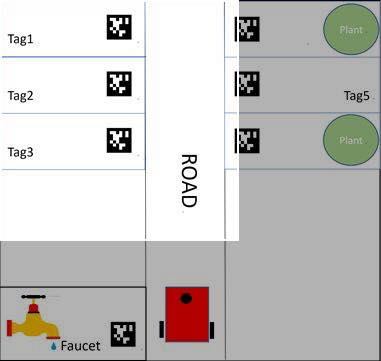
\includegraphics[width=0.8\columnwidth]{23602259_1745798205444844_1157434552_n.jpg}
\centering
\caption{illustration of the project}
\end{figure}


\section{SYSTEM ARCHITECTURE \& EQUIPMENTS}



\subsection{SYSTEM ARCHITECTURE}


\begin{figure}[htbp] % t means put this image at the top 
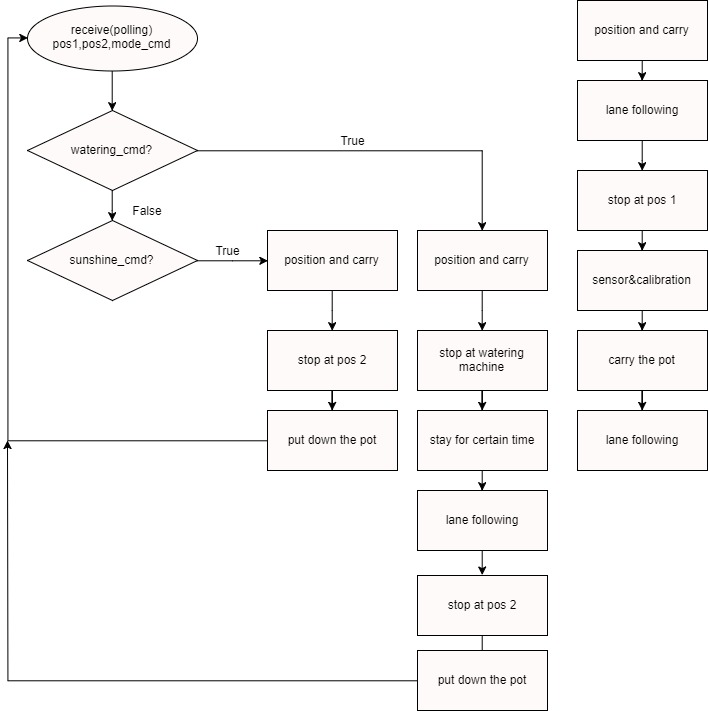
\includegraphics[width=0.8\columnwidth]{car_flowchart.jpg}
\centering
\caption{flow chart of duckiebot}
\end{figure}

\begin{figure}[htbp] % t means put this image at the top 
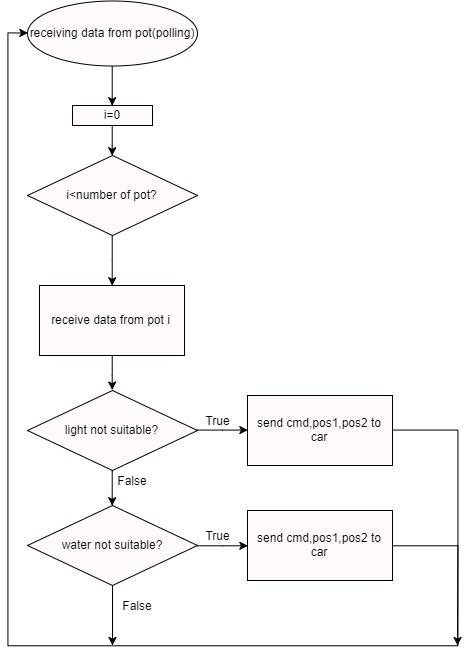
\includegraphics[width=0.8\columnwidth]{CmdServer_flowchart.jpg}
\centering
\caption{flow chart of control system}
\end{figure}

\hspace*{4mm}In this project, we will apply some Iot sensors and communication technology, ROS system including lane following, vision recognition, and some mechanical structure into the car and the watering machine. Our main idea is to accomplish an intellectual system which can replace the workload of taking care of the plant. The main control system will receive data from 6 pots in a room. These pots will transmit the information of light and humidity of the plant to the central control system. After receiving data, the control system will judge whether the status of the pot is suitable or not? If the status is not acceptable according to our database. The control system will call duckiebot to move to the certain position of the pot and carry it for watering at watering machine or take it to the place that the sunshine is suitable for the plant. Also, the system will collect all the data from the pot for more detailed information. \\
\hspace*{4mm}To simplify the problem, we will construct a fixed lane and watering machine for our cars. Next to the lane, there are 6 pot positions. All these positions contain a sticker with Apriltags on the ground. Therefore, our camera are able to recognize it and record the 3D position. \\





\begin{figure}[htbp] % t means put this image at the top 
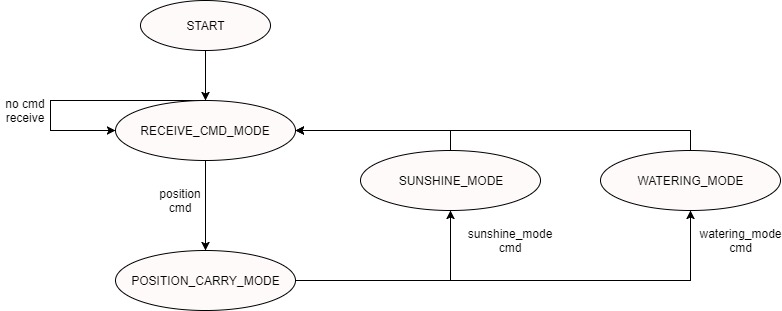
\includegraphics[width=0.8\columnwidth]{car_fsm.jpg}
\centering
\caption{FSM of duckiebot}
\end{figure}





\subsection{EQUIPMENTS} 

\begin{itemize}
\item XYZ robot arm*3(compatible with the potted plants metioned below)
\item Duckiebot*6
\item UV sensor (GY-ML8511)*6
\item Temperature and moisture sensor*4
\item plastic potted plants *6
\item Wifi router + YUN Arduino*6
\item stepper motors*2
\item Solenoid valve*2
\item Infrared sensor *1
\item color tape (white, yellow, red)
\item water tank*1
\item hemp rope
\item Apriltag*6
\item high-performance camera
\end{itemize}






\section{SPECIFIC AIMS}



\begin{itemize}
\item path planning and control
\end{itemize}


\begin{figure}[htbp] % t means put this image at the top 
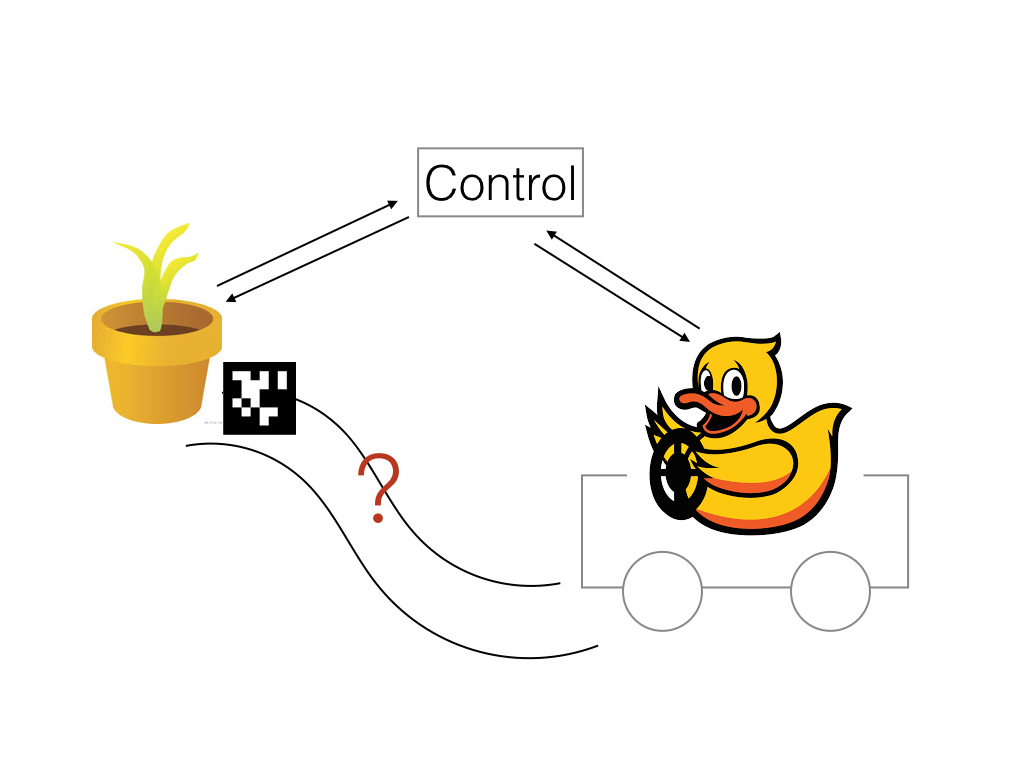
\includegraphics[width=0.8\columnwidth]{csp-aim-scenario.jpg}
\centering
\caption{scenario illustration of path planning and control}
\end{figure}


The bot will drive on a desired path, for moving the plants to a proper place (with sufficient sunlight and water).\\

\section{APPROACH}

\begin{itemize}
\item path planning and control
\end{itemize}


Several Apriltags will be placed, and each Apriltag coresponds to a plant behind it.

The bot will follow a lane with Apriltags.

A central control system will manege all the bots.

The bot will move a specific plant when receives command from the central control system, and report after completion.

We are able to plan the path of the bot, with the position and directions of the bot.

\section{SCHEDULE AND TEAM COLLABORATION}

\begin{itemize}
\item watering machine with communication part:12/7
\item UV sensor, humidity sensor + Bluetooth communication:12/7
\item control system:12/21
\item duckiebot lane following and vision recognition:12/21
\item mechanical arm control: 12/21
\end{itemize}
   

\addtolength{\textheight}{-12cm}   % This command serves to balance the column lengths
                                  % on the last page of the document manually. It shortens
                                  % the textheight of the last page by a suitable amount.
                                  % This command does not take effect until the next page
                                  % so it should come on the page before the last. Make
                                  % sure that you do not shorten the textheight too much.

\bibliographystyle{IEEEtran}
\bibliography{egbib}

\end{document}